\documentclass[10pt]{article}
\usepackage[T1]{fontenc}
\usepackage[utf8]{inputenc}
\usepackage[romanian]{babel}
\usepackage{tikz}
\usepackage{mathtools}
\usepackage{pgfplots}
\usepackage{amsthm,amsmath,amssymb}
\usepackage{graphicx}
\usepackage{parskip}
\setlength{\parindent}{0pt}

\newcommand*{\QED}{\hfill\ensuremath{\square}}%

\title{CSCI 6342 Module 7}
\author{Courtney Duquettte}
\date{11 April 2018}

\begin{document}
	\maketitle
	
	\textbf{\large Exercise 1:}\\
	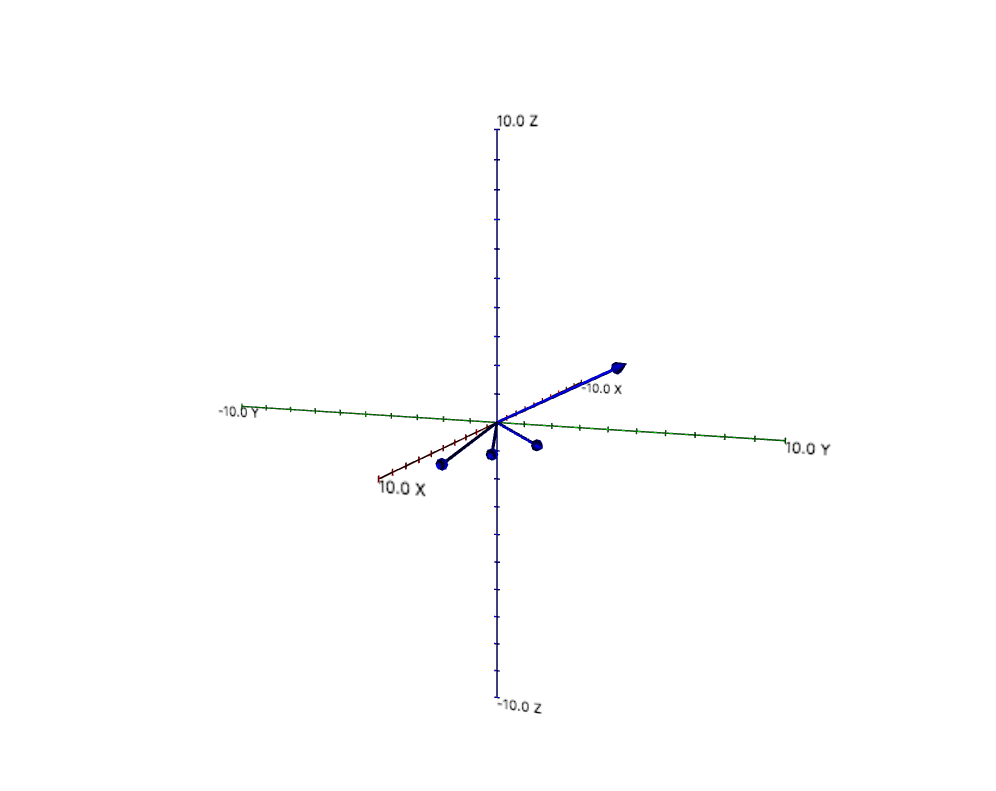
\includegraphics[scale=0.2]{module7_exercise1}
	\\
	
	\textbf{\large Exercise 2:}\\
	$c_3$ is not included in the linear combination because it is linearly dependent on the other two columns. \\
	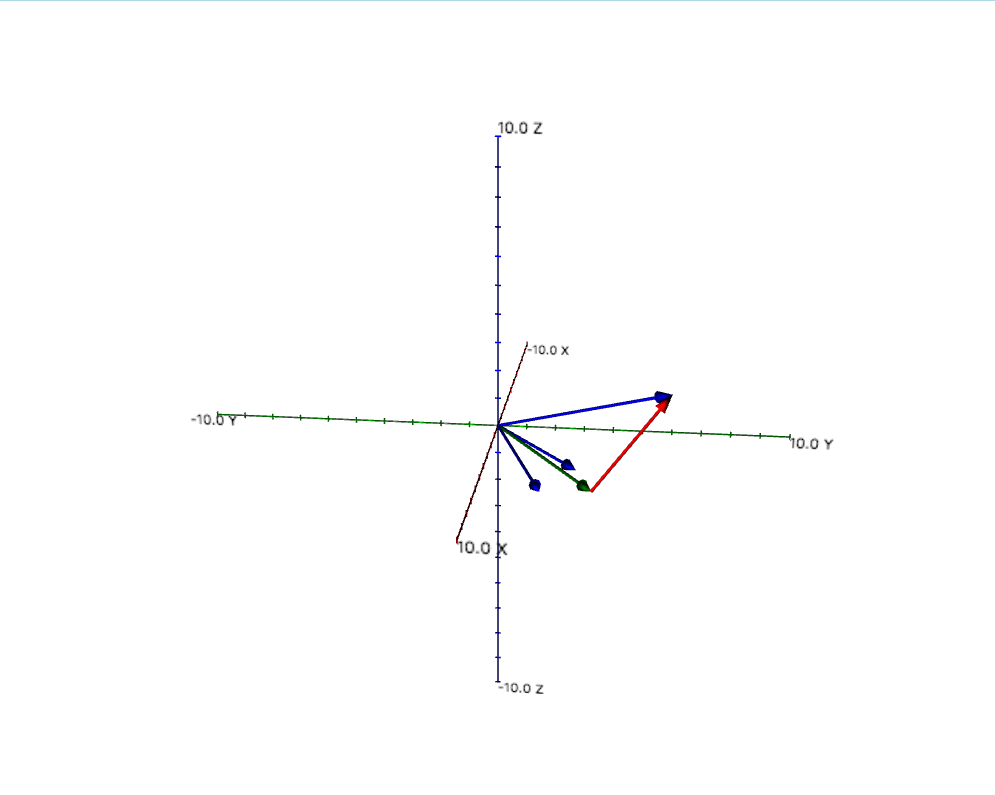
\includegraphics[scale=0.2]{module7_exercise2_1}\\
	If I increase the range, I get a $y$ vector that is a bit closer, in the sense that it is the same as $b$, but without the $z$ component. \\
	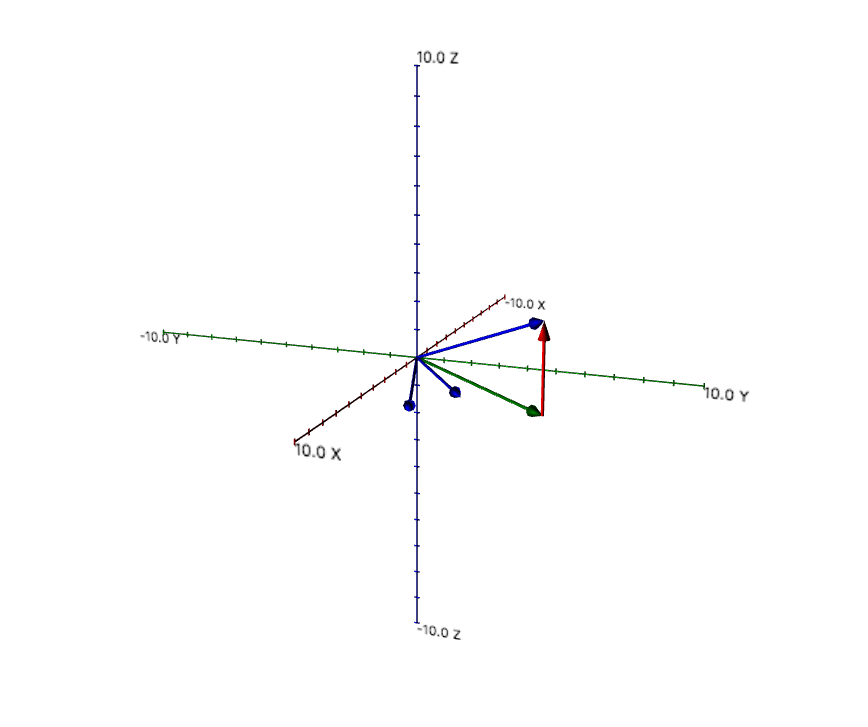
\includegraphics[scale=0.2]{module7_exercise2_new_range}
	\\
	
	\textbf{\large Exercise 3:}\\
	We need to show that $AB < AC$ for all $AC$. We know that 
	\begin{alignat*}{2}
		AB^2 + BC^2 &= AC^2\\
		AB^2 &= AC^2 - BC^2\\
		AB^2 &< AC^2\\
		AB &< AC
	\end{alignat*}
	So, the shortest distance from the point to the plane is on the perpendicular to the plane.
	\\
	
	\textbf{\large Exercise 4:}\\
	Both $c_1$ and $c_2$ are in the $xy$-plane, with $z$ components of 0. So, the closest linear combination of them to $b$ will be the projection of $b$ on the $xy$-plane. Therefore, if we look at $\textbf{z}$, the vector form $y$ to $b$, since it is orthogonal to the projection, it is orthogonal to both $c_1$ and $c_2$.
	\\
	
	\textbf{\large Exercise 5:}\\
	Using the data in the example above and taking the dot product, the equations for $\alpha$ and $\beta$ are
	$$\begin{array}{lllllll}
	42 - 40\alpha - 30\beta &= 0\\
	38 - 30\alpha -25\beta &= 0
	\end{array}$$
	and by solving these equations, we get $\alpha = \frac{-27}{30}$ and $\beta = \frac{13}{5}$. \\
	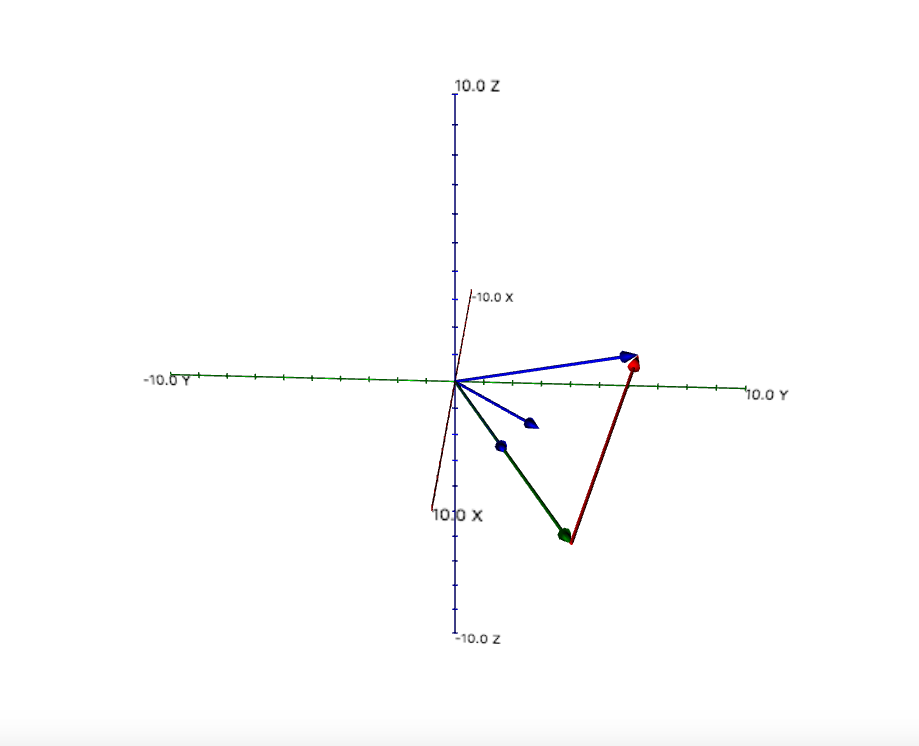
\includegraphics[scale=0.2]{module7_exercise5}
	\\
	
	\textbf{\large Exercise 6:}\\
	This works because of matrix multiplication. By have the $c$'s as rows, we are going to multiply each $c_i$ with $z_i$. 
	\\
	
	\textbf{\large Exercise 7:}\\
	$B$ is the transpose of $A$. 
	\\
	
	\textbf{\large Exercise 8:}\\
	
	\textbf{\large Exercise 9:}\\
	$A \rightarrow (m \times n)$, $A^T \rightarrow (n \times m)$, $A^TA \rightarrow (n \times n)$. So, \\
	$$\begin{array}{lllllll}
		(A^TA)^{-1}A^Tb &\rightarrow& (n \times n)(n \times m)(m \times 1)\\
		&\rightarrow& (n \times m)(m \times 1)\\
		&\rightarrow& (n \times 1)
	\end{array}$$
	
	\textbf{\large Exercise 10:}\\
	\begin{alignat*}{2}
		(A^TA)^{-1} &= A^{-1}(A^T)^{-1}\\
		(A^TA)^{-1}A^T &= A^{-1}(A^T)^{-1}A^T\\
		(A^TA)^{-1}A^T &= A^{-1}\\
		(A^TA)^{-1}A^Tb &= A^{-1}b
	\end{alignat*}
	
	\textbf{\large Exercise 11:}\\
	If $\textbf{A}^{-1}$ exists, the dimension and the column rank are equal. Since those two are equal, the row rank is also equal to the other two. This means that is $\textbf{A}^{-1}$ exists, then $\left(\textbf{A}^{T}\right)^{-1}$ must also exist.
	\\
	
	\textbf{\large Exercise 12:}\\
	We have $AB^{-1} = B^{-1}A^{-1}$. Now, in exercise 10, if we replace $A^T$ with $A$ and $A$ with $B$, then we can use the same proof to prove Theorem 7.1. 
	\\
	
	\textbf{\large Exercise 13:}\\\\
	Matrix (2x2):\\
	0.250 -0.300\\
	-0.300  0.400\\
	x[0]=-0.9000000000000004 x[1]=2.6000000000000014\\
	
	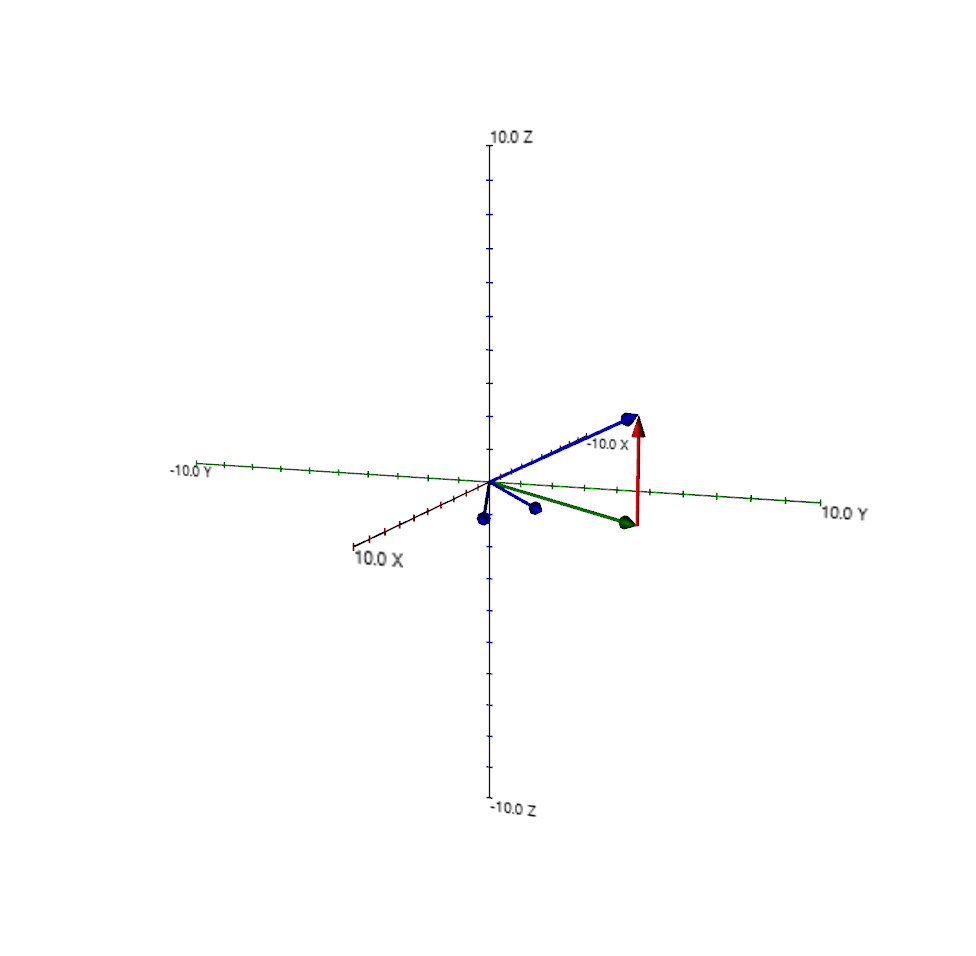
\includegraphics[scale=0.3]{module7_exercise13}
	\\
	
	\textbf{\large Exercise 14:}\\
	The columns is not linearly independent because no inverse exists.
	\\
	
	\textbf{\large Exercise 15:}\\
	\begin{tabular}{cc}
		Before: & After:\\ 
		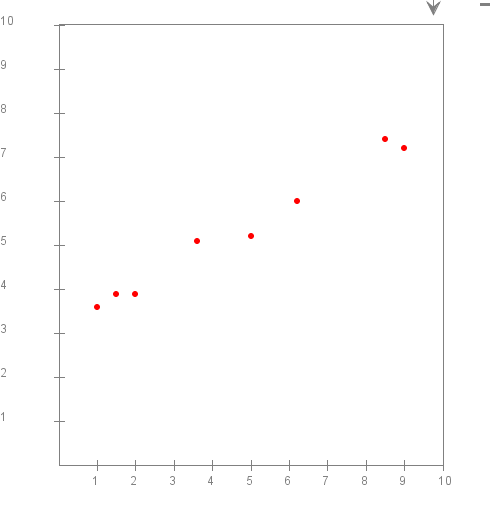
\includegraphics[scale=.3]{module7_exercise15_a} & 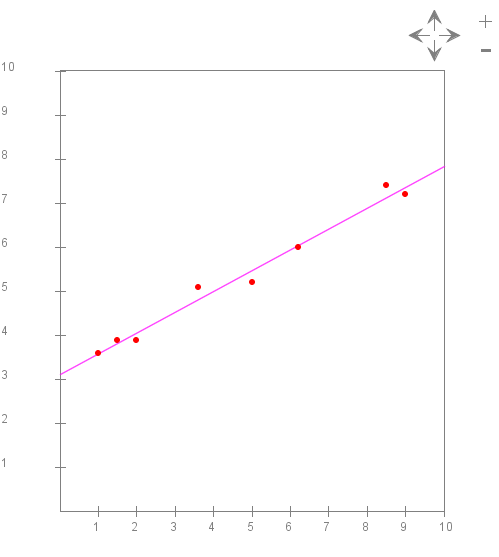
\includegraphics[scale=.3]{module7_exercise15_b}
	\end{tabular}
	
	\textbf{Console Output:} \\
	0.014788524105294281 -0.06802721088435369\\
	-0.06802721088435368 0.43792517006802695\\
	xhat[0]=0.47219757468204593 xhat[1]=3.115391156462591\\
	xhat[0]=0.47219757468204593 xhat[1]=3.115391156462591
	\\
	
	\textbf{\large Exercise 16:}\\
	\begin{tabular}{cc}
		Before: & After:\\ 
		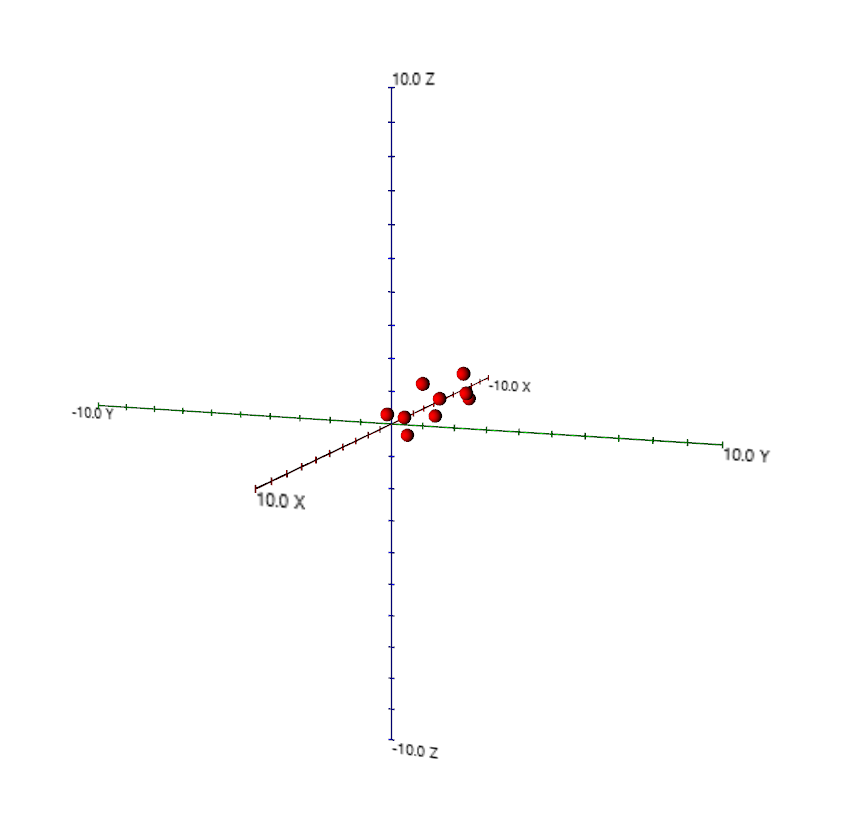
\includegraphics[scale=.3]{module7_exercise16_a} & 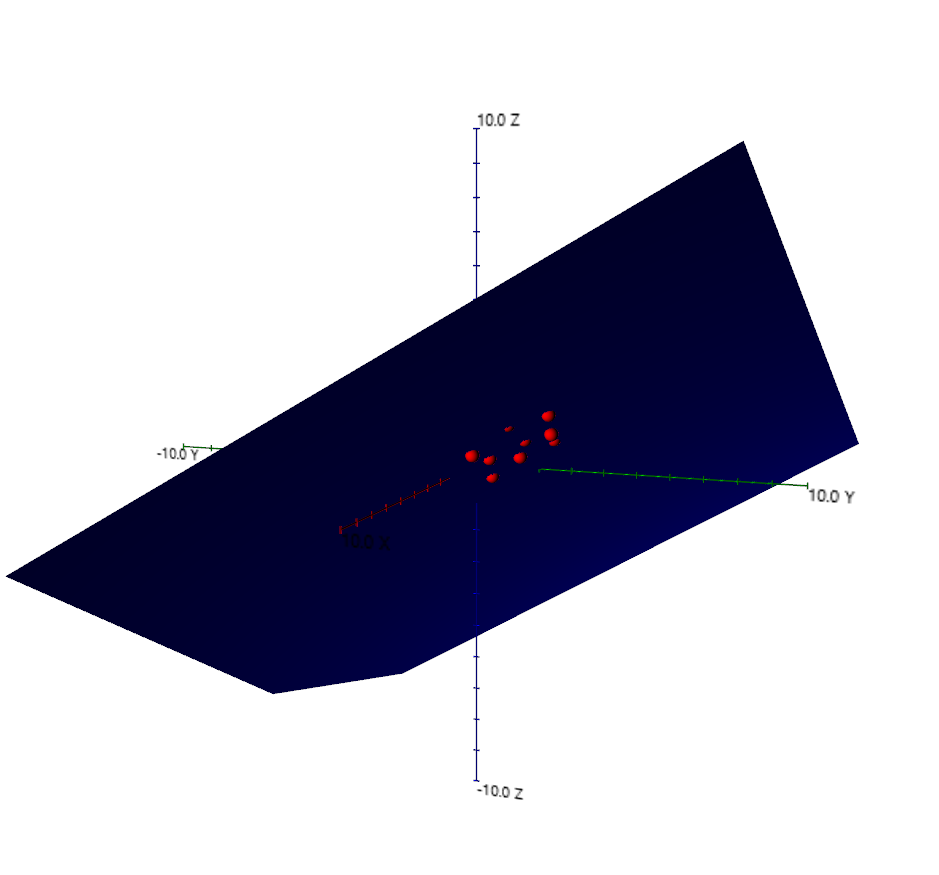
\includegraphics[scale=.3]{module7_exercise16_b}
	\end{tabular}
	
	\textbf{xhat}:\\
	-0.49850399194963124 -0.5828317907131417 -1.1785831129209399
	\\
	
	\textbf{\large Exercise 17:}\\
	\begin{tabular}{cc}
		Before: & After:\\
		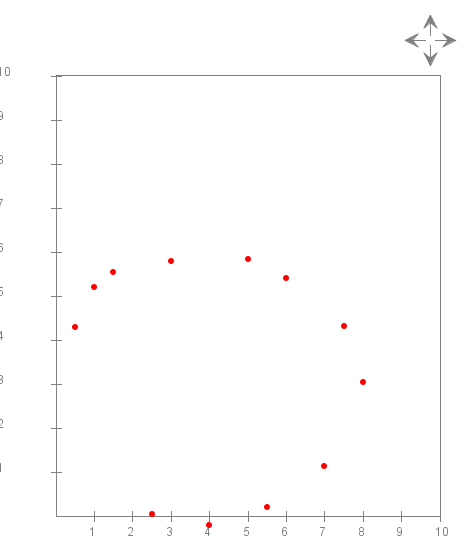
\includegraphics[scale=.5]{module7_exercise17} & 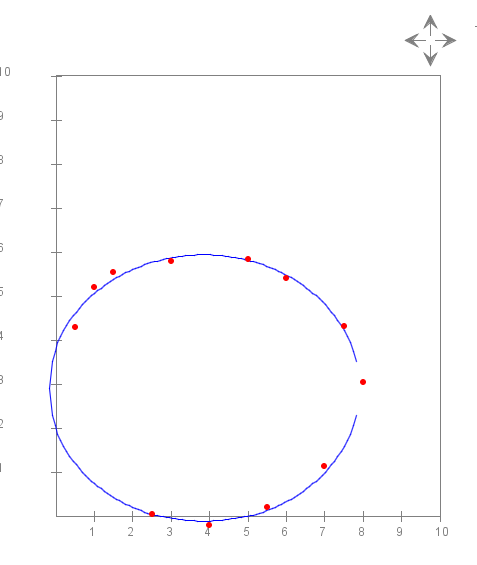
\includegraphics[scale=.5]{module7_exercise17_b}
	\end{tabular}
	
	\textbf{\large Exercise 18:}\\
	Before change of basis:\\
	meanX= 4.462, meanY= 4.575 varX= 5.846, varY= 6.505 covariance=49.260
	\\\\
	After change of basis:\\
	meanX= 4.519, meanY= 0.056 varX= 6.166, varY= 0.009 covariance= 1.319
	\\
	
	\textbf{\large Exercise 19:}\\
	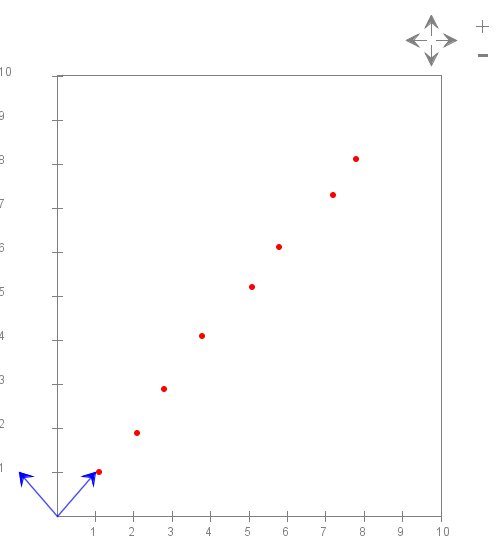
\includegraphics[scale=.5]{module7_exercise19}
	\\\\
	Coordinates after change of basis:\\
	( 1.050, -0.050)\\
	( 2.000, -0.100)\\
	( 2.850,  0.050)\\
	( 3.950,  0.150)\\
	( 5.150,  0.050)\\
	( 5.950,  0.150)\\
	( 7.250,  0.050)\\
	( 7.950,  0.150)
	\\
	
	\textbf{\large Exercise 20:}\\
	$$ \alpha = \frac{\textbf{w} \cdot \textbf{v}}{\textbf{v} \cdot \textbf{v}} = \frac{(4)(6) + (3)(2)}{(6)(6) + (2)(2)} = \frac{30}{40} = \frac{3}{4}$$
	$$ \textbf{z} = \begin{bmatrix}4 \\ 3\end{bmatrix} - \frac{3}{4}\begin{bmatrix}6 \\ 2\end{bmatrix} = \begin{bmatrix}-0.5 \\ 1.5\end{bmatrix}$$
	$$ \textbf{z} \cdot \textbf{v} = (-0.5)(6) + (1.5)(2) = 0$$
	\\
	
	\textbf{\large Exercise 21:}\\
	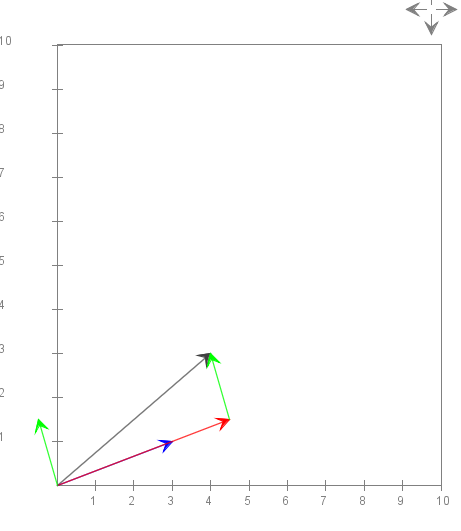
\includegraphics[scale=.5]{module7_exercise21}
	\\\\
	alpha = 1.5\\
	z=(-0.5,1.5)\\
	z dot v = 0.0\\
	\\\\
	The additional arrow is $\textbf{z}$.
	\\
	
	\textbf{\large Exercise 22:}\\
	\begin{tabular}{cc}
		Before: & After:\\
		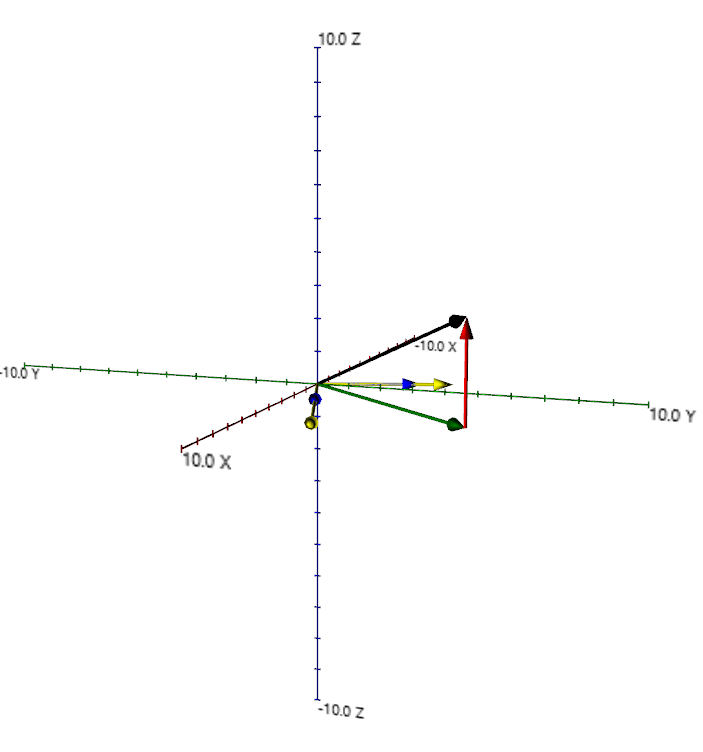
\includegraphics[scale=.4]{module7_exercise22_a} & 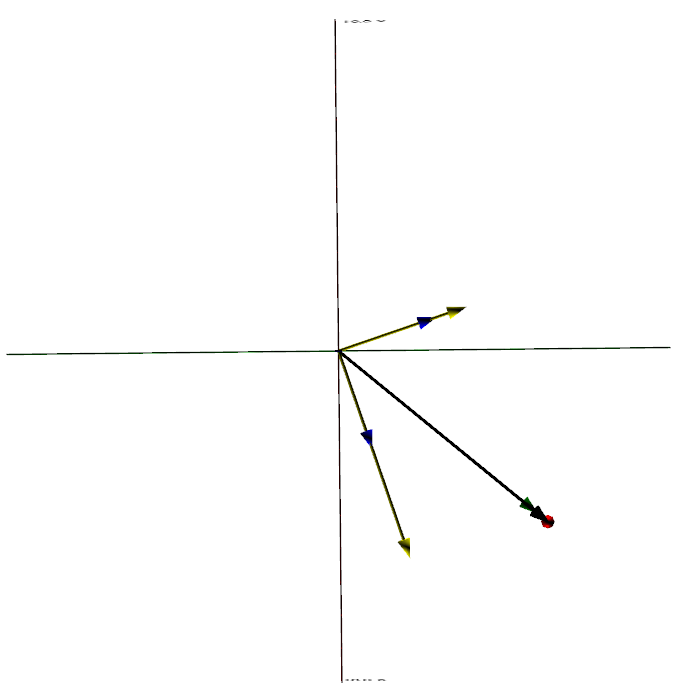
\includegraphics[scale=.4]{module7_exercise22_b}
	\end{tabular}
	
	z dot v1 = -2.6645352591003757E-15\\
	z dot v2 = 8.881784197001252E-16
	\\
	
	\textbf{\large Exercise 23:}\\
	\begin{itemize}
		\item $\textbf{v}_1 \cdot \textbf{v}_2 = (6)(-1) + (2)(3) = 0$	
		\item $\alpha_1 = \frac{(4)(6) + (2)(3)}{(6)(6) + (2)(2)} = .75$ and $\alpha_2 = \frac{(4)(-1) + (3)(3)}{(-1)(-1) + (3)(3)} = .5$
		\item $\text{proj}_{v_1} = .75 \begin{bmatrix}6\\2\end{bmatrix} = \begin{bmatrix}\frac{9}{2}\\\frac{3}{2}\end{bmatrix}$ and $\text{proj}_{v_2} = .5 \begin{bmatrix}-1\\3\end{bmatrix} = \begin{bmatrix}-\frac{1}{2}\\\frac{3}{2}\end{bmatrix}$
		\item $\textbf{w} = \begin{bmatrix}\frac{9}{2}\\\frac{3}{2}\end{bmatrix} + \begin{bmatrix}-\frac{1}{2}\\\frac{3}{2}\end{bmatrix} = \begin{bmatrix}4\\3\end{bmatrix}$
	\end{itemize}
	
	\textbf{\large Exercise 24:}\\
	
	\textbf{\large Exercise 25:}\\
	
	\textbf{\large Exercise 26:}\\\\
	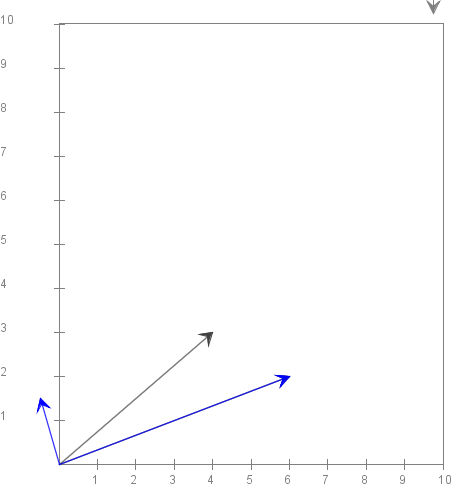
\includegraphics[scale=.5]{module7_exercise26}
	
	\textbf{\large Exercise 27:}\\
	\begin{tabular}{cc}
		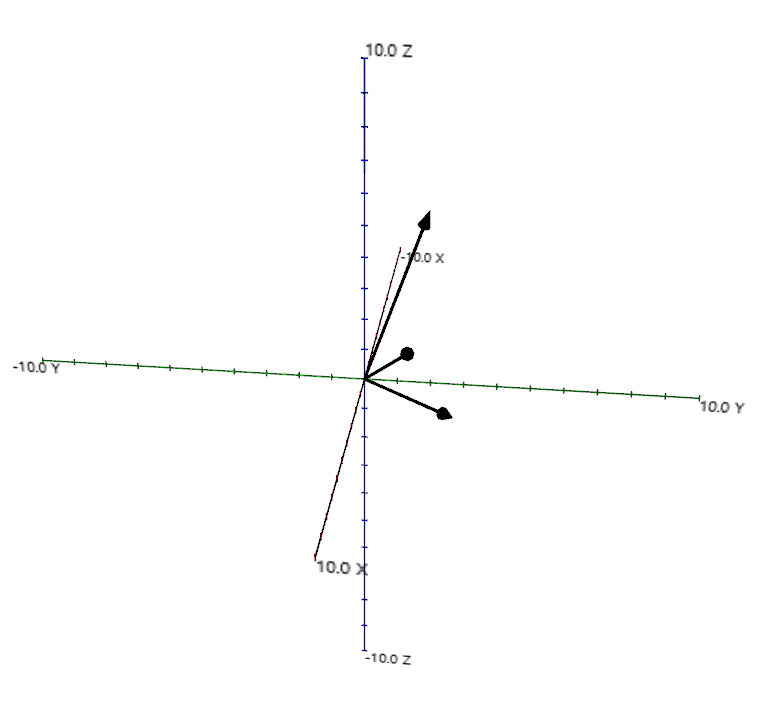
\includegraphics[scale=.4]{module7_exercise27} & 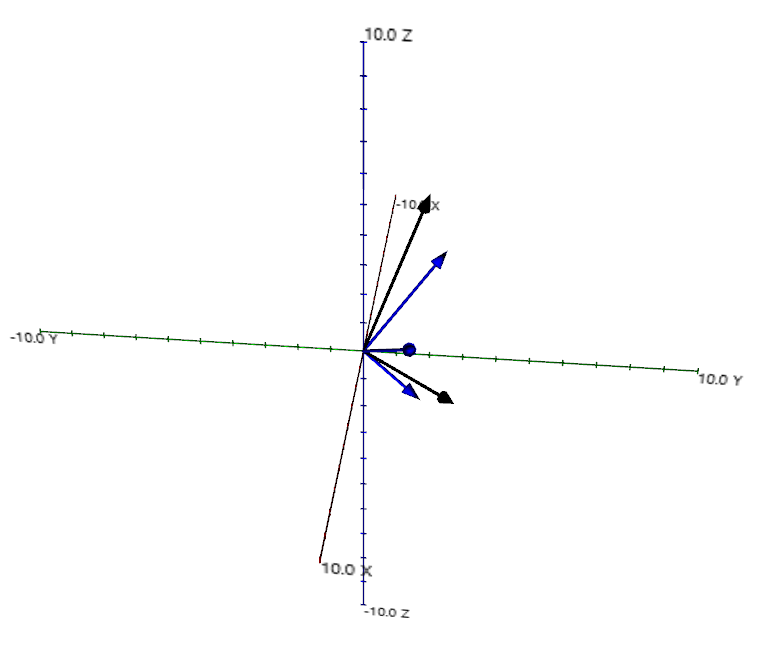
\includegraphics[scale=.4]{module7_exercise27_b}
	\end{tabular}
	
	v1 dot v2 = 3.552713678800501E-15\\
	v1 dot v3 = 5.329070518200751E-15\\
	v2 dot v3 = -3.552713678800501E-15
	\\
	
	\textbf{\large Exercise 28:}\\
	
	\textbf{\large Exercise 29:}\\
	
	\textbf{\large Exercise 30:}\\
	
	\textbf{\large Exercise 31:}\\
	
	\textbf{\large Exercise 32:}\\
	
	\textbf{\large Exercise 33:}\\
	
	\textbf{\large Exercise 34:}\\
	
\end{document}